\section{Priority Inheritance Protocol}

\subsection{Definition}

$C(R_{k})\stackrel{def}{=}\underset{h}{\mathrm{max}} \{P_{h}| \tau_{h} uses R_{k}\}  $

\ref{fig:pip}
\begin{figure}[h]
    \centering
    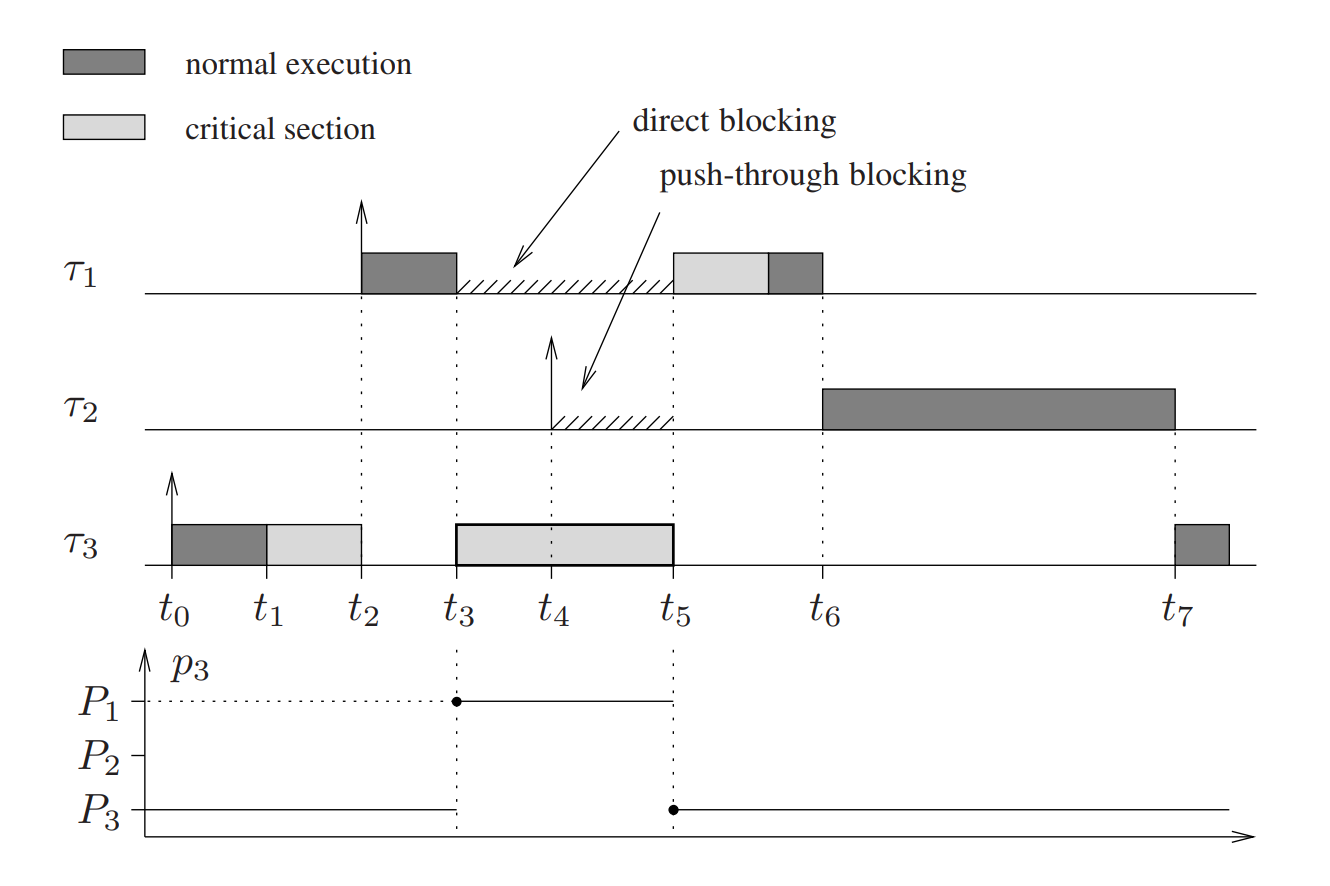
\includegraphics[width=0.5\textwidth]{pip}
    \caption{Example of Priority Inheritance Protocol. \cite{b5}}
    \label{fig:pip}
\end{figure}

\ref{fig:pip_nested}
\begin{figure}[h]
    \centering
    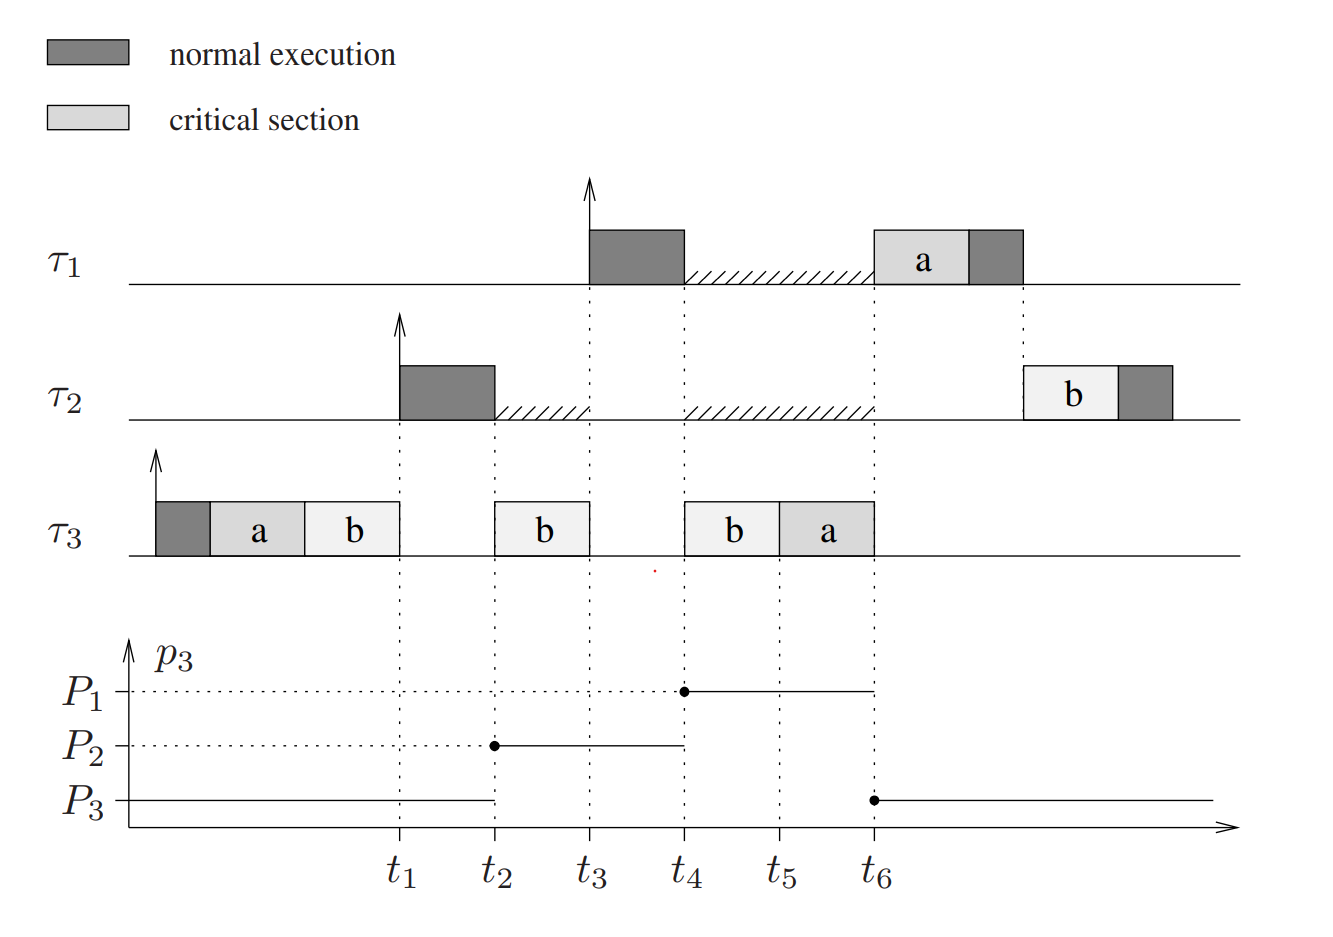
\includegraphics[width=0.5\textwidth]{pip_nested}
    \caption{Priority inheritance with nested critical sections.\cite{b5}}
    \label{fig:pip_nested}
\end{figure}

\ref{fig:tpi}
\begin{figure}[h]
    \centering
    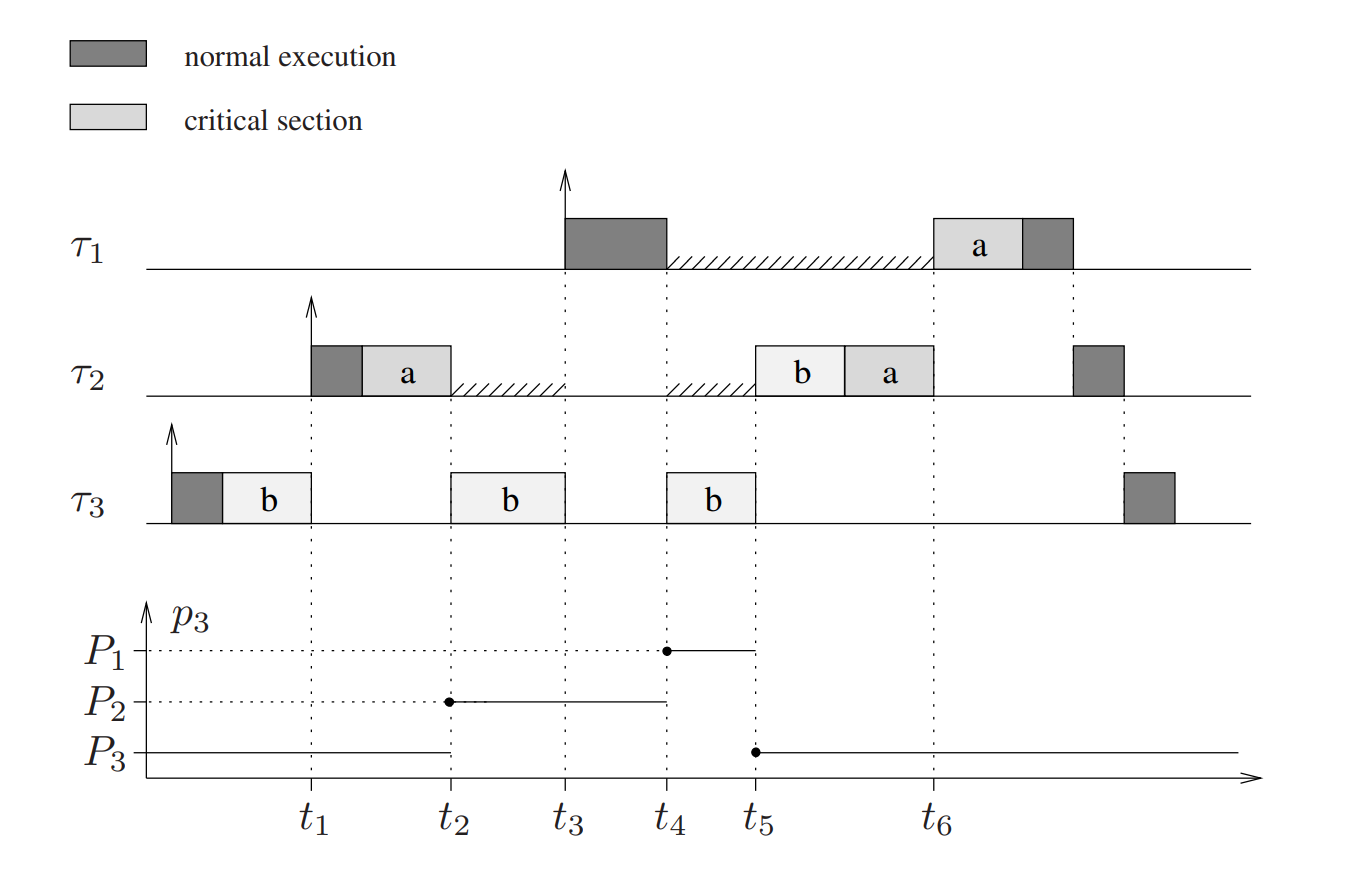
\includegraphics[width=0.5\textwidth]{tpi}
    \caption{Example of transitive priority inheritance.\cite{b5}}
    \label{fig:tpi}
\end{figure}

\subsection{Blocking Time computation}

$ \sigma \frac{dir}{i,j} =  \sigma_{i} \cap \sigma_{j} $

$ \sigma \frac{pt}{i,j} =  \underset{h:P_{h}>P_{i}}{\cup} \sigma_{h} \cap \sigma_{j} $


 $ \sigma_{i,j} = \sigma \frac{dir}{i,j}\cup\sigma \frac{pt}{i,j} =  \underset{h:P_{h}>P_{i}}{\cup} \sigma_{h} \cap \sigma_{j} $

$ \gamma_{i,j}=\{Z_{j,k} | P_{j}<P_{i} and R_{k}\in \sigma_{i,j} \} $

$ \sigma_{i} =\underset{j:P_{j}>P_{i}}{\cup} \gamma_{i,j}$


$ B \frac{l}{i} =\sum_{j=i+1}^{n} \underset{k}{\mathrm{max}} \{\sigma_{j,k}-1| C(S_{k})\geq P_{i}\}$

$ B_{i} =\underset{j,k}{\mathrm{max}} \{\delta_{j,k}-1| Z_{j,k}\in \gamma_{i}\}$

$ \gamma_{1}=\{\} $

\subsection{Problem Arise}


\subsubsection{Chained Blocking}

\ref{fig:Example_of_chained_blocking}
\begin{figure}[h]
    \centering
    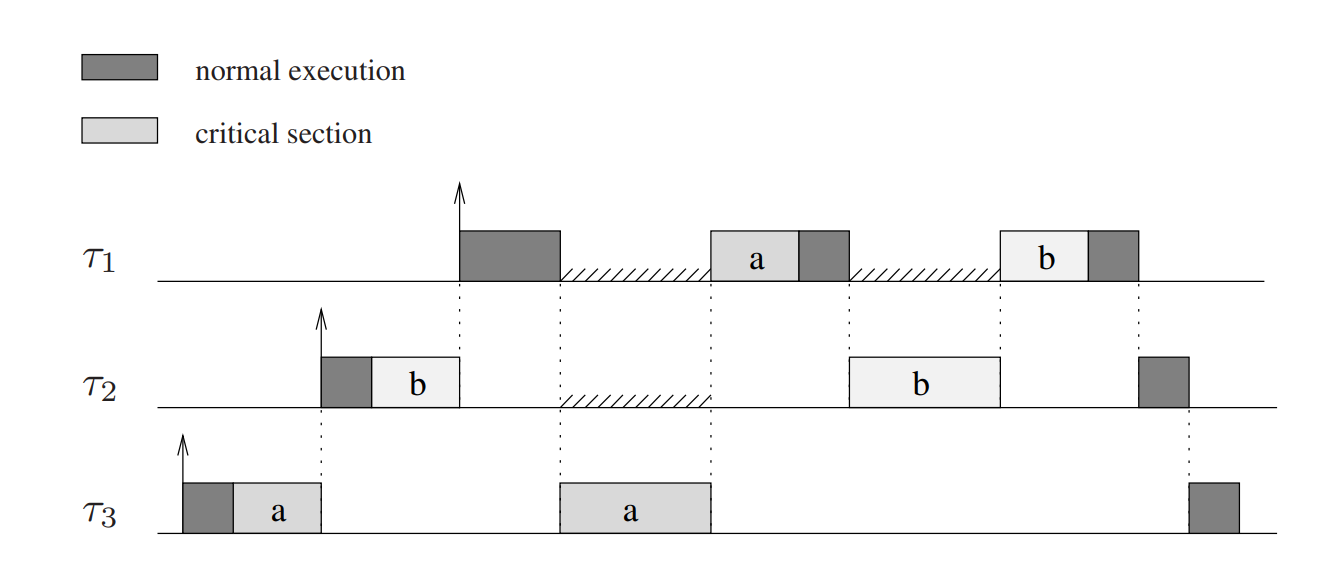
\includegraphics[width=0.5\textwidth]{Example_of_chained_blocking}
    \caption{Example of chained blocking.\cite{b5}}
    \label{fig:Example_of_chained_blocking}
\end{figure}

\subsubsection{Deadlock}

\ref{fig:Example_of_deadlock}
\begin{figure}[h]
    \centering
    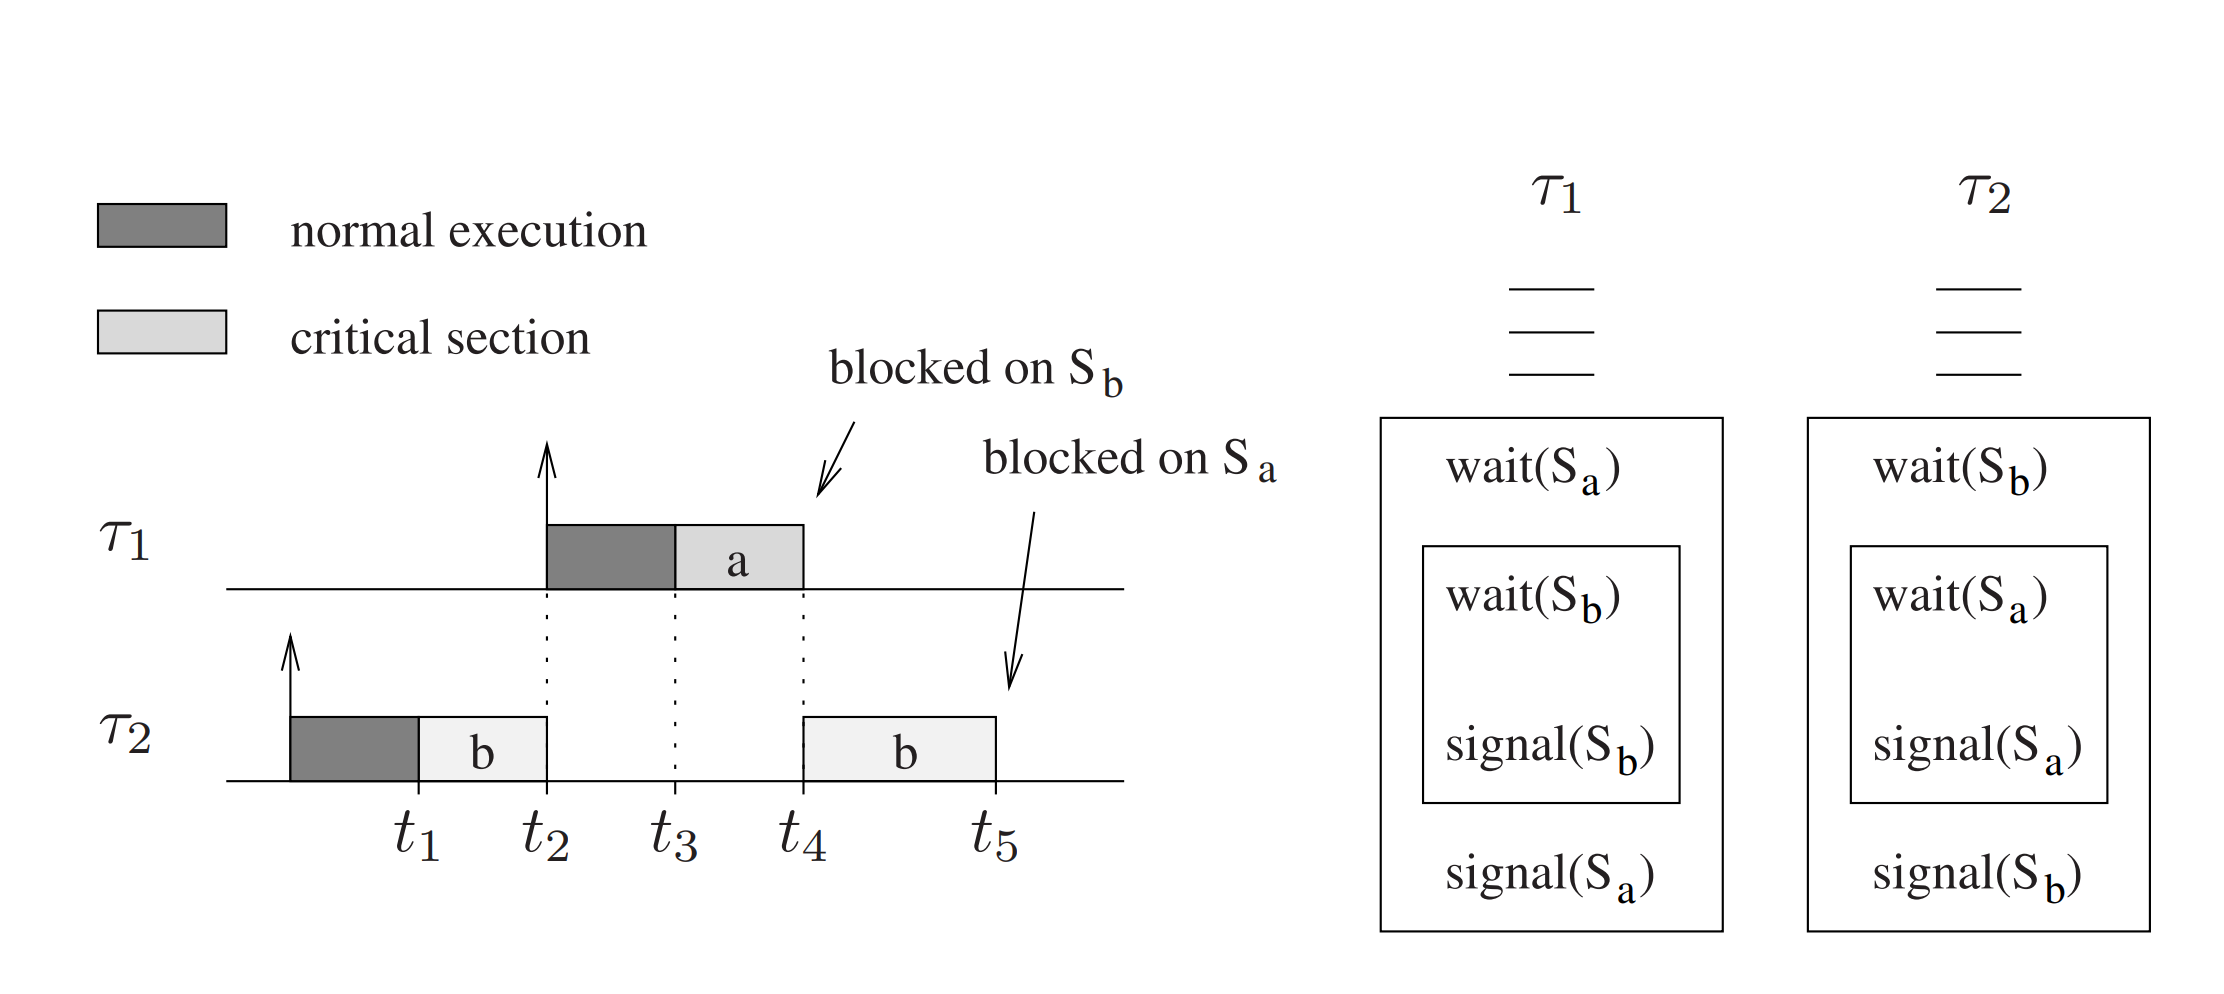
\includegraphics[width=0.5\textwidth]{Example_of_deadlock}
    \caption{Example of deadlock.\cite{b5}}
    \label{fig:Example_of_deadlock}
\end{figure}

















